\section{Project Area}
The Project Area is defined in order to manage in the best way the resources for the Project's lifecycle. All the Business process in this area aim to satisfy a part of the ``productive chain'' related to the Software environment and illustrated by the Software Engeenering discipline. The major aim of the area is to regroup each activity directly correlated with the Project to simplify the working procedure.

In this area there are several responsible, above all there is the Analyst who lead the practical Project develop, but parallel there is the Project Manager that need to achieve the better planning of the resources to improve the general efficiency. The charge may be covered by the same person. Other interesting roles are that which appear in the Working team organization unit illustrated on figure \ref{2img:working}; there may be several working team composed by upon two or more people and that works in a specific facet of the project.


\subsection{Requirement analysis}
\label{subsec:requirement}
The ``Requirement analysis'' business process aims to represent, through a finite sequence of step, the delicate task of gathering and formatting customers' requests in order to facilitate the following tasks. This process can be viewed as a manner of standardizing the incoming order whose natural language expressivity can be misunderstanded.

Except for the Requirement gathering subprocess, whose responsible is the representative, all the activities listed in figure \ref{2img:requirement} are supervised by the Analyst who should use his skills and experience to strongly manage at best each process' step.

\begin{figure}[ht!]
\begin{centering}
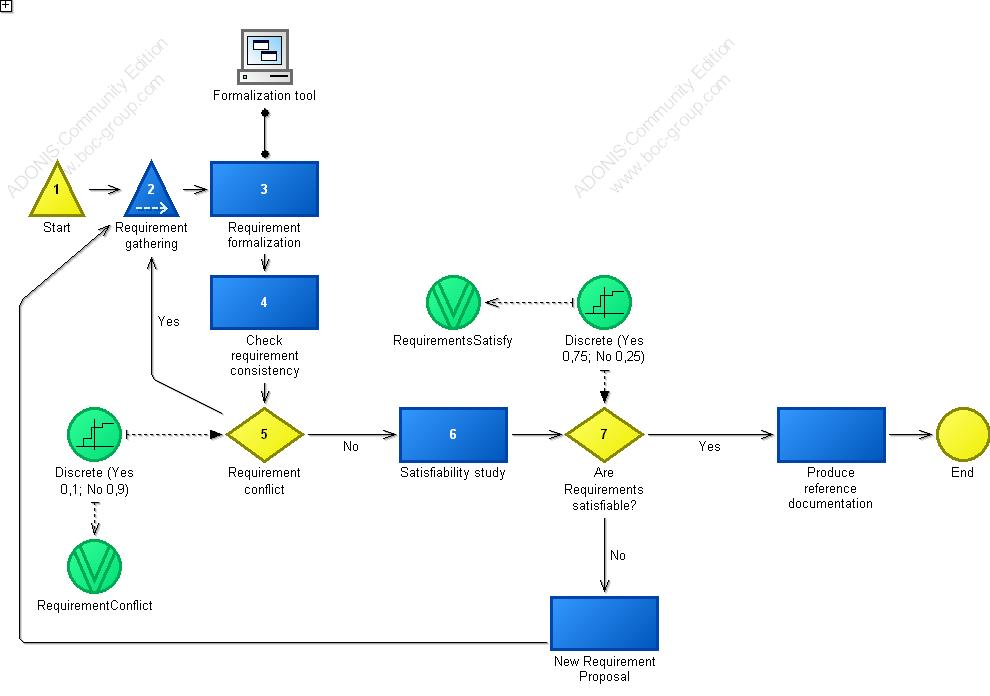
\includegraphics[scale=0.50, angle=90]{assign2/adonis/imgs/requirement.jpg}
\caption{AllSpark Requirement analysis.}
\label{2img:requirement}
\end{centering}
\end{figure}


\subsubsection{Path Analysis}
The path analysis procedure returns twenty-one distinct paths with the maximum probability of 67,10\% for the one reported straightward. The simplicity of the model came from the header of the path analysis shown next since the cycle time is actual the sum of all times.

\begin{alltt}
Probability:   67,1000\%
Execution time:  00:000:07:20:00
Waiting time:  00:000:00:00:00
Resting time:  00:000:00:00:00
Transport time:  00:000:00:30:00
Cycle time:  00:000:07:50:00
Costs:  2,000000

Requirement Analysis 0.1 (Business process model)
========================================
Process start: Start
Subprocess: Requirement gathering
Activity: Requirement formalization
Activity: Check requirement consistency
Decision: Requirement conflict --> RequirementConflict = 'No'
Activity: Satisfiability study
Decision: Are Requirements satisfiable? --> RequirementsSatisfy = 'Yes'
Activity: Produce reference documentation
End: End

Requirement Analysis 0.1 (Business process model) --> Requirement gathering 1 (Business process model)
========================================
Process start: Start
Activity: Requirement gathering
End: End
\end{alltt}


\subsubsection{Capacity Analysis}
The capacity analysis doesn't reveal any interesting information.

\begin{landscape}
\begin{table}
\centering
{\tiny
\begin{tabular}{|l|l|l|l|l|l|l|}
Business process&Activity&Performer&Number&Execution time&Cycle time&Costs\\
\hline
Requirement Analysis 0.3&&&&00:000:09:19:01&00:000:09:49:01&2,720800\\
\hline
&Requirement formalization &&1,488000&00:000:01:29:17&&1,190400\\
\hline
&&Analyst &1,488000&00:000:01:29:17&&1,190400\\
\hline
&Satisfiability study &&1,338000&00:000:02:40:34&&0,535200\\
\hline
&&Analyst &1,338000&00:000:02:40:34&&0,535200\\
\hline
&Check requirement consistency &&1,488000&00:000:01:14:24&&0,595200\\
\hline
&&Analyst &1,488000&00:000:01:14:24&&0,595200\\
\hline
&Produce reference documentation &&1,000000&00:000:03:00:00&&0,400000\\
\hline
&&Analyst &1,000000&00:000:03:00:00&&0,400000\\
\hline
&New Requirement Proposal &&0,338000&00:000:00:10:08&&0,000000\\
\hline
&&Analyst &0,338000&00:000:00:10:08&&0,000000\\
\hline
&Requirement gathering &&1,488000&00:000:00:44:38&&0,000000\\
\hline
&&Representative &1,488000&00:000:00:44:38&&0,000000\\
\hline
Total&&&&00:000:09:19:01&&2,720800
\end{tabular}
}
\caption{Capacity analysis for Requirement analysis.}
\end{table}
\end{landscape}
%

%

\subsection{Desing/Planning project}
The ``Design/Planning project'' business process aim to represent the deterministic stage required for start the project. Since is a common standardize phase, is obviusly without any decision point since all the constitutive activities are needed and well defined. 

The Path analysis is so useless and it will skipped.

\begin{figure}[ht!]
\begin{centering}
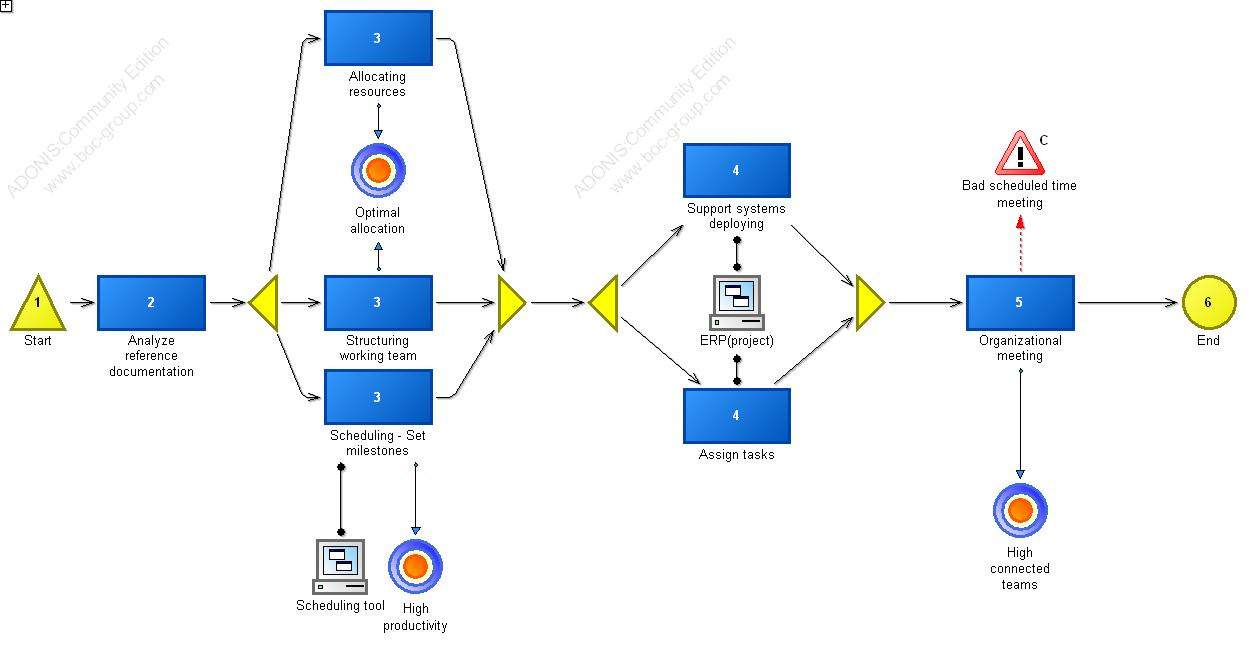
\includegraphics[scale=0.50, angle=90]{assign2/adonis/imgs/design.jpg}
\caption{AllSpark Design/Planning project.}
\label{2img:desing}
\end{centering}
\end{figure}


\subsubsection{Capacity Analysis}
The capacity analysis permits to see each activity behaviour. Particula interesting is the difference between Execution time and the Cycle time that reveals the efficiency of parallelization of activities which permits, in this case, a gain of working hours.

\begin{landscape}
\begin{table}
\centering
{\tiny
\begin{tabular}{|l|l|l|l|l|l|l|}
Business process&Activity&Performer&Number&Execution time&Cycle time&Costs\\
\hline
Design/Planning Project 0.1&&&&00:000:07:00:00&00:000:04:30:00&32,400000\\
\hline
&Analyze reference documentation &&1,000000&00:000:01:00:00&&0,800000\\
\hline
&&Analyst &1,000000&00:000:01:00:00&&0,800000\\
\hline
&Structuring working team &&1,000000&00:000:01:00:00&&0,400000\\
\hline
&&Area Manager &1,000000&00:000:01:00:00&&0,400000\\
\hline
&Allocating resources &&1,000000&00:000:01:00:00&&0,500000\\
\hline
&&Area Manager &1,000000&00:000:01:00:00&&0,500000\\
\hline
&Scheduling - Set milestones &&1,000000&00:000:02:00:00&&30,000000\\
\hline
&&Analyst &1,000000&00:000:02:00:00&&30,000000\\
\hline
&Assign tasks &&1,000000&00:000:00:30:00&&0,200000\\
\hline
&&Analyst &1,000000&00:000:00:30:00&&0,200000\\
\hline
&Support systems deploying &&1,000000&00:000:01:00:00&&0,500000\\
\hline
&&Area Manager &1,000000&00:000:01:00:00&&0,500000\\
\hline
&Organizational meeting &&1,000000&00:000:00:30:00&&0,000000\\
\hline
&&Area Manager &1,000000&00:000:00:30:00&&0,000000\\
\hline
Total&&&&00:000:07:00:00&&32,400000
\end{tabular}
}
\caption{Capacity analysis for Design/Planning project.}
\end{table}
\end{landscape}
%

%

\subsection{Implementation}
The ``Implementation'' business process is the core of the Project Area intends that lot of time spend during the developing of a project is inside here. It is pretty difficult to evaluate with parameters since the complexity of some solution are strongly dependent on the scoper required by the customer and so it directed dependent by the Requirement Analysis described at page \pageref{subsec:requirement}. This process aim to generalize the procedure each developer should follow for own work.

Accordingly with figure \ref{2img:implementation}, the great major of the activities have the Programmer as direct responsible, but final one is supervised by the Analyst who is the only one can evaluate the work done.

\begin{figure}[ht!]
\begin{centering}
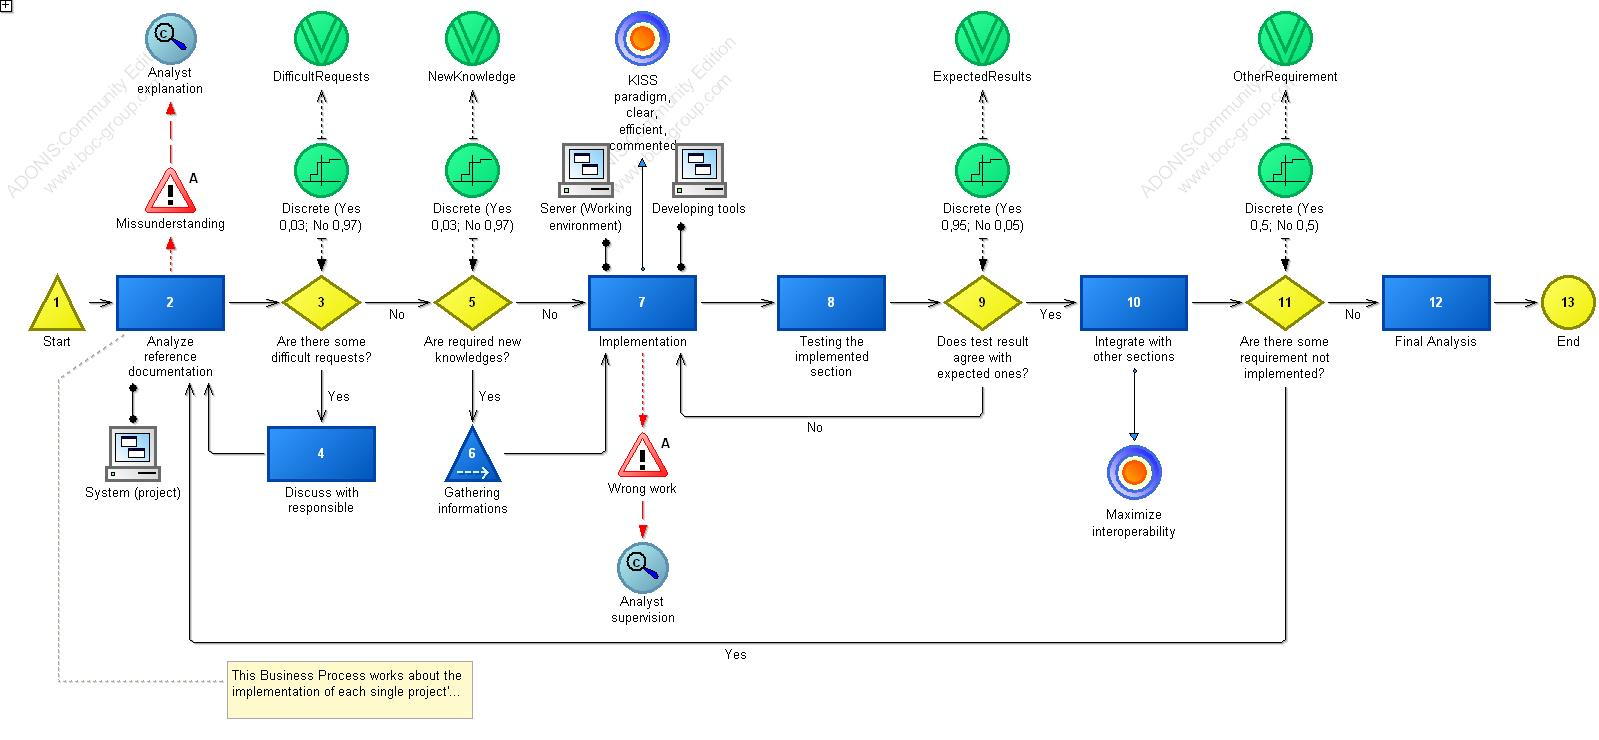
\includegraphics[scale=0.30, angle=90]{assign2/adonis/imgs/implementation.jpg}
\caption{AllSpark Implementation.}
\label{2img:implementation}
\end{centering}
\end{figure}


\subsubsection{Path Analysis}
The path analysis reveals several possible paths, lot of them don't have a relevant probability. To first two are very interesting since the execution time is completely different as shown in the table below. The second one shows what happen if the Programmer doesn't recognize the correct features representation assigned to him.

\begin{table}
\centering
\begin{tabular}{|l|l|l|l|l|}
Path&Probability&Execution time&Cycle time&Costs\\
\hline
1&0,5890&00:000:05:20:00&00:000:05:50:00&1,60\\
\hline
2&0,1760&00:001:00:25:00&00:001:01:25:00&3,2
\end{tabular}
\end{table}

\begin{alltt}
Probability:   58,9000\%
Execution time:  00:000:05:20:00
Waiting time:  00:000:00:05:00
Resting time:  00:000:00:25:00
Transport time:  00:000:00:00:00
Cycle time:  00:000:05:50:00
Costs:  1,600000

Implementation 0.1 (Business process model)
========================================
Process start: Start
Activity: Analyze reference documentation
Decision: Are there some difficult requests? --> DifficultRequests='No'
Decision: Are required new knowledges? --> NewKnowledge='No'
Activity: Implementation
Activity: Testing the implemented section
Decision: Does test result agree with expected ones? --> ExpectedResults='Yes'
Activity: Integrate with other sections
Decision: Are there some requirement not implemented? --> OtherRequirement='No'
Activity: Final Analysis
End: End
\end{alltt}

\begin{alltt}
Probability:   17,6000\%
Execution time:  00:001:00:25:00
Waiting time:  00:000:00:10:00
Resting time:  00:000:00:50:00
Transport time:  00:000:00:00:00
Cycle time:  00:001:01:25:00
Costs:  3,200000

Implementation 0.1 (Business process model)
========================================
Process start: Start
Activity: Analyze reference documentation
Decision: Are there some difficult requests? --> DifficultRequests='No'
Decision: Are required new knowledges? --> NewKnowledge='No'
Activity: Implementation
Activity: Testing the implemented section
Decision: Does test result agree with expected ones? --> ExpectedResults='Yes'
Activity: Integrate with other sections
Decision: Are there some requirement not implemented? --> OtherRequirement='Yes'
Activity: Analyze reference documentation
Decision: Are there some difficult requests? --> DifficultRequests='No'
Decision: Are required new knowledges? --> NewKnowledge='No'
Activity: Implementation
Activity: Testing the implemented section
Decision: Does test result agree with expected ones? --> ExpectedResults='Yes'
Activity: Integrate with other sections
Decision: Are there some requirement not implemented? --> OtherRequirement='No'
Activity: Final Analysis
End: End
\end{alltt}



\subsubsection{Capacity Analysis}
This capacity analyssi represent the characteristic of each activity in order to evaluate possibile strategy. The process is referred to only one developer or working unit.

\begin{landscape}
\begin{table}
\centering
{\tiny
\begin{tabular}{|l|l|l|l|l|l|l|}
Business process&Activity&Performer&Number&Execution time&Cycle time&Costs\\
\hline
Implementation 0.1&&&&00:000:08:33:36&00:000:09:22:27&3,018800\\
\hline
&Analyze reference documentation &&1,601000&00:000:00:48:02&&1,280800\\
\hline
&&Programmer &1,601000&00:000:00:48:02&&1,280800\\
\hline
&Discuss with responsible &&0,061000&00:000:00:00:55&&0,000000\\
\hline
&&Programmer &0,061000&00:000:00:00:55&&0,000000\\
\hline
&Implementation &&1,635000&00:000:06:32:24&&1,308000\\
\hline
&&Programmer &1,635000&00:000:06:32:24&&1,308000\\
\hline
&Testing the implemented section &&1,635000&00:000:00:24:32&&0,000000\\
\hline
&&Programmer &1,635000&00:000:00:24:32&&0,000000\\
\hline
&Integrate with other sections &&1,540000&00:000:00:30:48&&0,000000\\
\hline
&&Programmer &1,540000&00:000:00:30:48&&0,000000\\
\hline
&Final Analysis &&1,000000&00:000:00:15:00&&0,000000\\
\hline
&&Analyst &1,000000&00:000:00:15:00&&0,000000\\
\hline
&Gathering informations &&0,043000&00:000:00:01:56&&0,430000\\
\hline
&&Programmer &0,043000&00:000:00:01:56&&0,430000\\
\hline
Total&&&&00:000:08:33:36&&3,018800
\end{tabular}
}
\caption{Capacity analysis for Implementation.}
\end{table}
\end{landscape}
%

%

\subsection{Project Deployment}
The ``Project Deployment'' business process is the set of activities required to enable the product to customer. In particular the meaning of the task is to transfer the developing project from a programming environment to a public environment such as the server or, may be, generating a retailer copy to distribuite. The main role of the task is to realize the deployment with the less number of issues in order to gain time and prevent future modify, so testing the Product is very important.

There are several activities which need the collaboration of both Programmer and Sysadmin. The supervision is charged on the Analyst whose authority assure good interoperability trhough teams.

\begin{figure}[ht!]
\begin{centering}
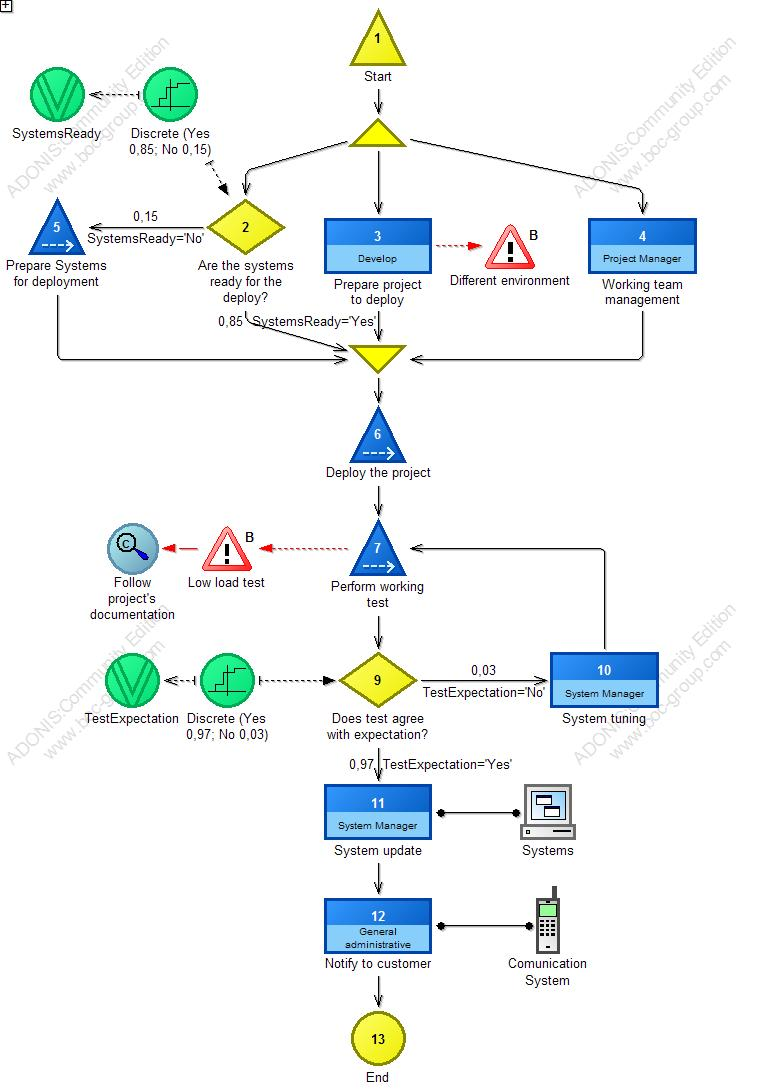
\includegraphics[scale=0.50]{assign2/adonis/imgs/deploy.jpg}
\caption{AllSpark Project Deployment.}
\label{2img:deploy}
\end{centering}
\end{figure}


\subsubsection{Path Analysis}
The path analysis reveals two important path represented in the following schemas. Particular interesting is the second one which represent the case of System not ready and so the process is delayed to prepare it to host the Product.

\begin{table}
\centering
\begin{tabular}{|l|l|l|l|l|}
Path&Probability&Execution time&Cycle time&Costs\\
\hline
1&0,8140&00:000:01:25:00&00:000:01:45:00&10,40\\
\hline
2&0,1510&00:000:02:55:00&00:000:03:28:00&11,4
\end{tabular}
\end{table}

\begin{alltt}
Probability:   81,4000\%
Execution time:  00:000:01:25:00
Waiting time:  00:000:00:10:00
Resting time:  00:000:00:00:00
Transport time:  00:000:00:10:00
Cycle time:  00:000:01:45:00
Costs:  10,400000

Deployment 0.1 (Business process model)
========================================
Process start: Start
Parallelity: Parallelity-21955
    *
    Activity: Prepare project to deploy
    *
    Activity: Working team management
    *
    Decision: Are the systems ready for the deploy? --> SystemsReady='Yes'
Merging: Merging-21962
Subprocess: Deploy the project
Subprocess: Perform working test
Decision: Does test agree with expectation? --> TestExpectation='Yes'
Activity: System update
Activity: Notify to customer
End: End

Deployment 0.1 (Business process model) --> Perform working test 1 (Business process model)
========================================
Process start: Start
Activity: Deploy project
End: End

Deployment 0.1 (Business process model) --> Deploy project 1 (Business process model)
========================================
Process start: Start
Activity: Deploy project
End: End
\end{alltt}


\subsubsection{Capacity Analysis}
The capacity analysis reveal the expected value about the possibility having a particular activity.

\begin{landscape}
\begin{table}
\centering
{\tiny
\begin{tabular}{|l|l|l|l|l|l|l|}
Business process&Activity&Performer&Number&Execution time&Cycle time&Costs\\
\hline
Deployment 0.1&&&&00:000:01:37:59&00:000:01:59:53&10,546000\\
\hline
&Prepare project to deploy &&1,000000&00:000:00:00:00&&0,000000\\
\hline
&&Programmer &1,000000&00:000:00:00:00&&0,000000\\
\hline
&Working team management &&1,000000&00:000:00:00:00&&0,000000\\
\hline
&&Area Manager &1,000000&00:000:00:00:00&&0,000000\\
\hline
&System tuning &&0,025000&00:000:00:00:00&&0,000000\\
\hline
&&Area Manager &0,025000&00:000:00:00:00&&0,000000\\
\hline
&System update &&1,000000&00:000:00:00:00&&0,000000\\
\hline
&&Area Manager &1,000000&00:000:00:00:00&&0,000000\\
\hline
&Notify to customer &&1,000000&00:000:00:00:00&&0,000000\\
\hline
&&Secretary &1,000000&00:000:00:00:00&&0,000000\\
\hline
&Deploy project &&1,000000&00:000:00:55:00&&10,000000\\
\hline
&&Analyst &1,000000&00:000:00:55:00&&10,000000\\
\hline
&Prepare systems &&0,136000&00:000:00:12:14&&0,136000\\
\hline
&&Area Manager &0,136000&00:000:00:12:14&&0,136000\\
\hline
&Deploy project &&1,025000&00:000:00:30:45&&0,410000\\
\hline
&&Analyst &1,025000&00:000:00:30:45&&0,410000\\
\hline
Total&&&&00:000:01:37:59&&10,546000
\end{tabular}
}
\caption{Capacity analysis for Deployment.}
\end{table}
\end{landscape}
%

%

\subsection{Project closure}
The ``Project closure'' business process is a formal procedure to terminate a Project. In particular a predefinited sequence of possible steps aims to achieve the best implicit gain from a concluded project in order to evaluate the experience done and so improve skills and methodology for next jobs.

A great part of activities are supervised, as common in this Area, by the Analyst who cover a important role to gather best value from the closing.

\begin{figure}[ht!]
\begin{centering}
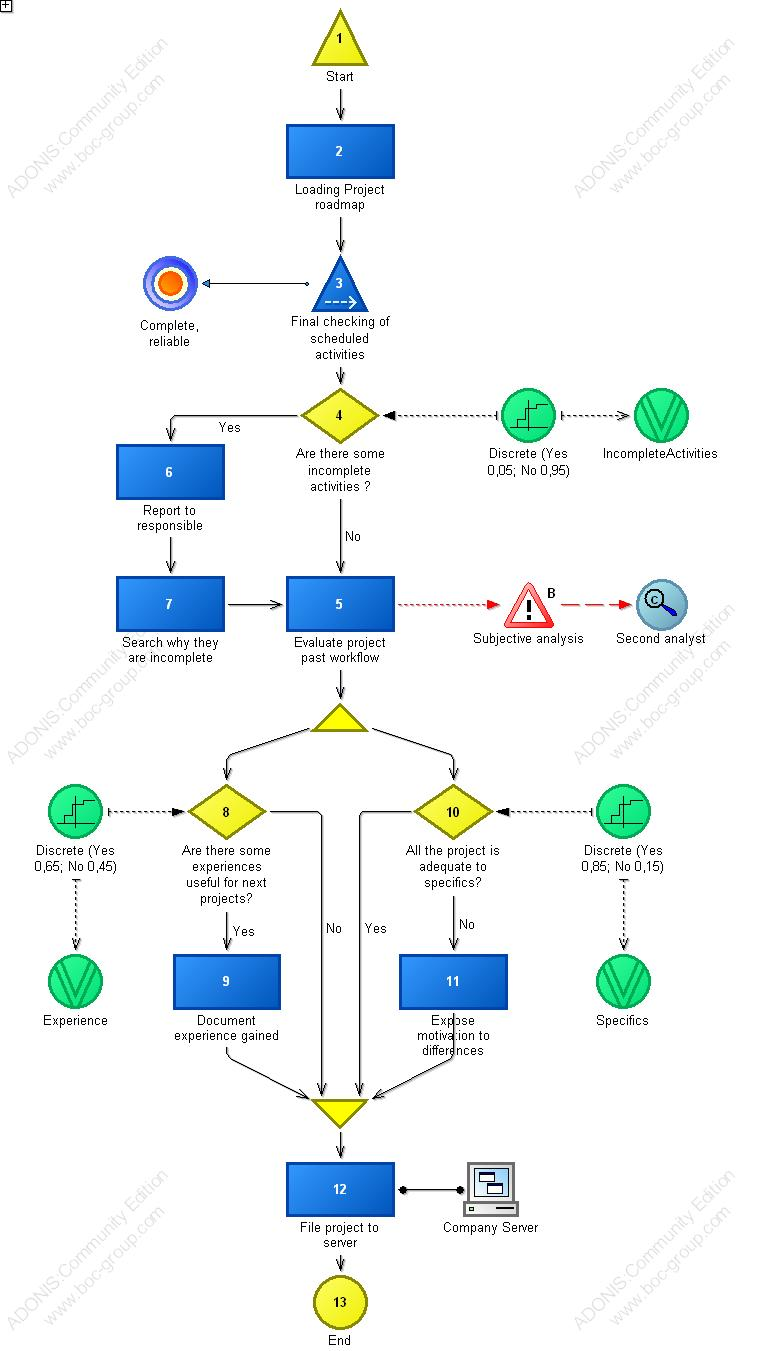
\includegraphics[scale=0.50]{assign2/adonis/imgs/closure.jpg}
\caption{AllSpark Project Closure.}
\label{2img:closure}
\end{centering}
\end{figure}


\subsubsection{Path Analysis}
There are seven different kind of relevant paths that the analysis reveals, two of them are presented in the table below. The less probable of the two is the cheaper in the timing consuming measurement of all the seven, so both paths are presented straight forward the table.

\begin{table}
\centering
\begin{tabular}{|l|l|l|l|l|}
Path&Probability&Execution time&Cycle time&Costs\\
\hline
1&0,5400&00:000:02:15:00&00:000:02:20:00&1,60\\
\hline
2&0,2800&00:000:01:25:00&00:000:01:30:00&0,8
\end{tabular}
\end{table}

\begin{alltt}
Probability:   54,0000\%
Execution time:  00:000:02:15:00
Waiting time:  00:000:00:00:00
Resting time:  00:000:00:00:00
Transport time:  00:000:00:05:00
Cycle time:  00:000:02:20:00
Costs:  1,600000

Project Closure 0.3 (Business process model)
========================================
Process start: Start
Activity: Loading Project roadmap
Activity: Final checking of scheduled activities
Decision: Are there some incomplete activities ? --> IncompleteActivities='No'
Activity: Evaluate project past workflow
Parallelity: Parallelity-22224
    *
    Decision: Are there some experiences useful for next projects? --> Experience='Yes'
    Activity: Document experience gained
    *
    Decision: All the project is adequate to specifics? --> Specifics='Yes'

Merging: Merging-22246
Activity: File project to server
End: End
\end{alltt}

\begin{alltt}
Probability:   17,8000\%
Execution time:  00:001:00:25:00
Waiting time:  00:000:00:10:00
Resting time:  00:000:00:50:00
Transport time:  00:000:00:00:00
Cycle time:  00:001:01:25:00
Costs:  3,200000

Implementation 0.3 (Business process model)
========================================
Process start: Start
Activity: Analyze reference documentation
Decision: Are there some difficult requests? --> DifficultRequests='No'
Decision: Are required new knowledges? --> NewKnowledge='No'
Activity: Implementation
Activity: Testing the implemented section
Decision: Does test result agree with expected ones? --> ExpectedResults='Yes'
Activity: Integrate with other sections
Decision: Are there some requirement not implemented? --> OtherRequirement='Yes'
Activity: Analyze reference documentation
Decision: Are there some difficult requests? --> DifficultRequests='No'
Decision: Are required new knowledges? --> NewKnowledge='No'
Activity: Implementation
Activity: Testing the implemented section
Decision: Does test result agree with expected ones? --> ExpectedResults='Yes'
Activity: Integrate with other sections
Decision: Are there some requirement not implemented? --> OtherRequirement='No'
Activity: Final Analysis
End: End
\end{alltt}



\subsubsection{Capacity Analysis}
The capacity analysis of this process doesn't reveal anything important except for the summary of the activities involved.

\begin{landscape}
\begin{table}
\centering
{\tiny
\begin{tabular}{|l|l|l|l|l|l|l|}
Business process&Activity&Performer&Number&Execution time&Cycle time&Costs\\
\hline
Project Closure 0.3&&&&00:000:02:03:15&00:000:02:05:31&1,428000\\
\hline
&Document experience gained &&0,642000&00:000:00:32:06&&0,513600\\
\hline
&&Programmer &0,642000&00:000:00:32:06&&0,513600\\
\hline
&Expose motivation to differences &&0,143000&00:000:00:04:17&&0,114400\\
\hline
&&Programmer &0,143000&00:000:00:04:17&&0,114400\\
\hline
&File project to server &&1,000000&00:000:00:15:00&&0,800000\\
\hline
&&Sysadmin &1,000000&00:000:00:15:00&&0,800000\\
\hline
&Loading Project roadmap &&1,000000&00:000:00:05:00&&0,000000\\
\hline
&&Area Manager &1,000000&00:000:00:05:00&&0,000000\\
\hline
&Report to responsible &&0,053000&00:000:00:00:48&&0,000000\\
\hline
&&Programmer &0,053000&00:000:00:00:48&&0,000000\\
\hline
&Search why they are incomplete &&0,053000&00:000:00:01:04&&0,000000\\
\hline
&&Analyst &0,053000&00:000:00:01:04&&0,000000\\
\hline
&Evaluate project past workflow &&1,000000&00:000:00:45:00&&0,000000\\
\hline
&&Analyst &1,000000&00:000:00:45:00&&0,000000\\
\hline
&Final checking of scheduled activities &&1,000000&00:000:00:20:00&&0,000000\\
\hline
&&Analyst &1,000000&00:000:00:20:00&&0,000000\\
\hline
Total&&&&00:000:02:03:15&&1,428000
\end{tabular}
}
\caption{Capacity analysis for Project closure.}
\end{table}
\end{landscape}
%

%